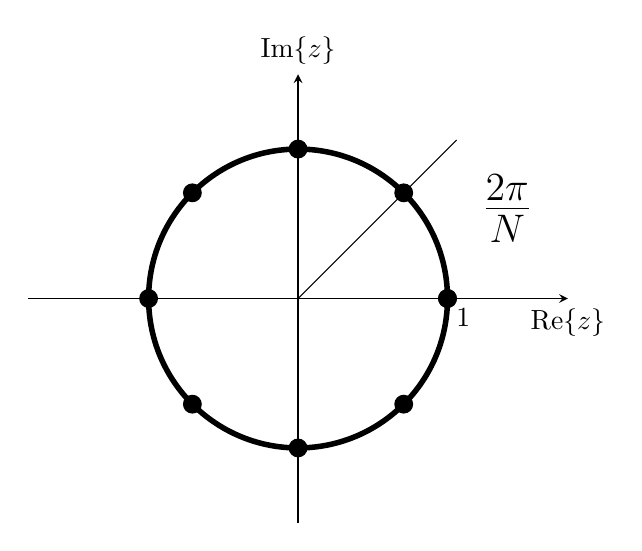
\begin{tikzpicture} 
\begin{axis}[
axis equal,
axis lines*=middle,
enlargelimits = false,
xmax=1.5,
xmin=-1.5,
ymin=-1.5,
ymax=1.5,
axis line style={->,>=stealth},
xlabel={$\mathrm{Re}\{z\}$},
ylabel={$\mathrm{Im}\{z\}$},
every axis x label/.style={
    at={(ticklabel* cs:1)},
    anchor=north,
},
every axis y label/.style={
    at={(ticklabel* cs:1)},
    anchor=south,
},
xtick={1},
ytick=\empty,
xticklabels={1},
%xmajorgrids,
%ymajorgrids,
xticklabel style = {xshift=+0.2cm},
every outer y axis line/.append style={white!15!black},
every y tick label/.append style={font=\color{white!15!black}},
legend style={draw=white!15!black,fill=white,legend cell align=left}]
%\pgfplotsinvokeforeach{0, 45,..., 360}{
%	\draw [black] (axis cs:0,0) -- (axis cs:{1.5*cos(#1)}, {1.5*sin(#1)});
%}
\draw [black] (axis cs:0,0) -- (axis cs:{1.5*cos(45)}, {1.5*sin(45)});
\draw[black, line width=2pt] (axis cs:0,0) circle [radius=1];
\draw [black, mark=*, mark size=3pt, only marks, thick,  domain=0:360, samples=9] plot ({cos(\x)}, {sin(\x)} );
%\draw[latex'-latex', double] (1.25,0) arc (0:45:1.25);
\node (z) at (axis cs: 1.4, 0.6) {\huge $\frac{2\pi}{N}$};
\end{axis}
\end{tikzpicture}
